\documentclass[12pt]{article}
\usepackage{graphicx}
\usepackage{amsmath}

\usepackage[margin=1in]{geometry}
\usepackage{float}
\usepackage{listings}
\usepackage{booktabs}

\title{Labwork 7: Reduction}
\author{Ngo Quang Truong 2540106}
\date{3 Oct 2026}

\begin{document}

\maketitle
\newpage

\section{Introduction}
This report presents a grayscale stretch implemented on GPU by combining the Map and Reduction patterns.

\section{Method}
The grayscale stretch has three steps:
\begin{enumerate}
    \item \textbf{Map}: convert each RGB pixel to gray, $g = (R+G+B)/3$ (2D kernel, $16\times16$ block).
    \item \textbf{Reduce}: find the minimum and maximum intensity of the gray image.
    \item \textbf{Map}: linearly stretch each pixel from $[min, max]$ to $[0, 255]$:
    \begin{equation}
    g' = \frac{g - min}{max - min} \times 255
    \end{equation}
\end{enumerate}
Test image: a $3840\times2160$ RGB image.

\section{Reduction}
The gray image is flattened to a 1D array and split into blocks of 256 threads.
\begin{itemize}
    \item Each thread copies one pixel into two shared-memory arrays (one for min, one for max).
    \item The block halves the stride at each step (\texttt{s = 128, 64, \dots, 1}); thread \texttt{t < s} keeps the min/max of \texttt{t} and \texttt{t + s}. This avoids branch divergence and bank conflicts.
    \item Thread 0 writes the block result to global memory.
    \item The few thousand block results are copied back and finished on the CPU with \texttt{min()} / \texttt{max()}.
\end{itemize}

The GPU result was checked against \texttt{numpy.min} and \texttt{numpy.max}.

\begin{figure}[H]
    \centering
    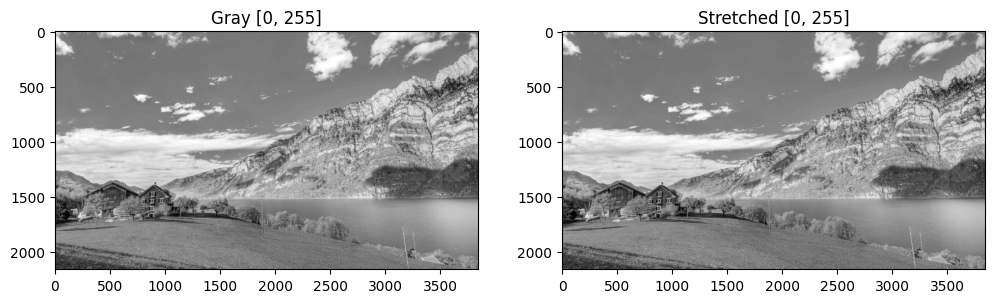
\includegraphics[width=\textwidth]{output.png}
    \caption{Gray image (left) vs.\ stretched output}
    \label{fig:stretch}
\end{figure}

\end{document}
